\section{0. Introduction}\label{introduction}

This project focuses on building a web application to predict house
prices for house buyers and house sellers.

The value of a house is more than just location and square footage.
Houses have several features that make up it's value.We are going to
take advantage of all the features to make accurate predictions about
the price of any house.

We developed our application using a series of logical steps to ensure
that users can easily use the application and make accurate predictions.

\begin{enumerate}
\def\labelenumi{\arabic{enumi})}
\setcounter{enumi}{-1}
\itemsep1pt\parskip0pt\parsep0pt
\item
  Introduction
\item
  Problem definition
\item
  Solution approach
\item
  Results and discussions
\item
  Conclusions
\item
  Refrences
\end{enumerate}

\section{1. Problem definition}\label{problem-definition}

We used a simple case study to understand the problem. There are two
clients at the same time without a conflict of intreset.

The house buyer, a client that wants to buy their dream home. They have
some locations in mind. Now, the client wants to know if the house price
matches the value. With the application, they can understand which
features are influence the final price. If the final price matches the
value predicted by the application the can ensure they are getting a
fair price.

The house seller, a client that buys houses, fixes them and then sells
houses to make profit. This client wants to take advantage of features
that influece the price of a house the most. They typically want to buy
a house at a low price and invest in features that will give the highest
return.

\section{2. Solution approach}\label{solution-approach}

\begin{enumerate}
\def\labelenumi{\arabic{enumi})}
\itemsep1pt\parskip0pt\parsep0pt
\item
  Define requirements
\item
  Gather data, analyze and build models
\item
  Build web backend API to use model
\item
  Design and develope frontend
\item
  Intergrate both frontend and backend
\item
  Test the entire application
\end{enumerate}

\subsection{Define requirements}\label{define-requirements}

The requriements were gathered from the problem and formally defined.

\subsubsection{User function}\label{user-function}

\begin{itemize}
\itemsep1pt\parskip0pt\parsep0pt
\item
  Predict house price
\item
  Customize house parameters
\item
  Assign unique label every prediction
\item
  Save recent predictions
\end{itemize}

\subsubsection{Operating enviroment}\label{operating-enviroment}

\begin{itemize}
\itemsep1pt\parskip0pt\parsep0pt
\item
  client/server system (Web)
\item
  client: Web browers
\item
  server: Python/Flask
\item
  database: sqlite
\item
  platform: Python/Javascript/HTML5/CSS3
\item
  Operating system: Windows, Mac, Linux
\end{itemize}

\subsection{2. Gather data, analyze and build
models}\label{gather-data-analyze-and-build-models}

We found an online kaggle challange that contained the data we needed to
solve the problem. Data was downloaded from
\href{https://www.kaggle.com/c/house-prices-advanced-regression-techniques/data}{here}
We broke everything into the following steps We started by loading data
and packages we needed for the research.We then analyzed the data to
understand the relationships between the price and other features. We
cleaned the data and using some domain knowlegde replaced some missing
values. The next step was feature tranformation to make the data
compatible with our models. We then trained our model and started
perfoming some predictions.

\subsection{3. Build web backend API to use
model}\label{build-web-backend-api-to-use-model}

Using python and the flask web framework we built a web API the takes
advantage of our model. The API comsumer can make a request containing
JSON map of features and their values. The flask server recieves this
request and sends a response containing the predicted price.

\subsection{6. Design and develope
frontend}\label{design-and-develope-frontend}

The User interface of the application was built using HTML, CSS3 and
javascript.

\subsection{7. Intergrate both frontend and
backend}\label{intergrate-both-frontend-and-backend}

Using the javascript, we send data from the forms on the webpage to the
flask server and the server sends a reponse, which is a prediction of
the price matching those features

\subsection{8. Test the entire
application}\label{test-the-entire-application}

We run multiple tests fixed bugs in the code.

\section{3. Results and discussions}\label{results-and-discussions}

\subsection{Screenshot of the
application}\label{screenshot-of-the-application}

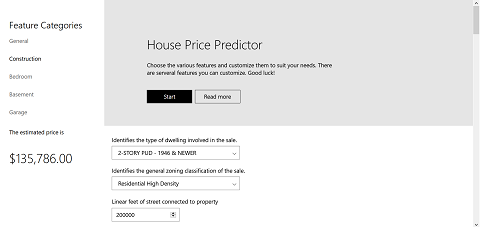
\includegraphics{images/screenshot-01.png}
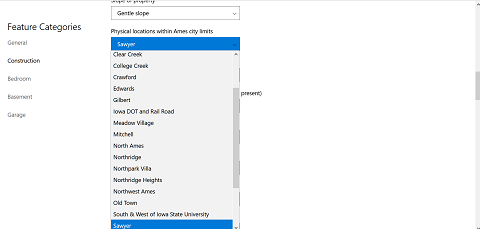
\includegraphics{images/screenshot-02.png}
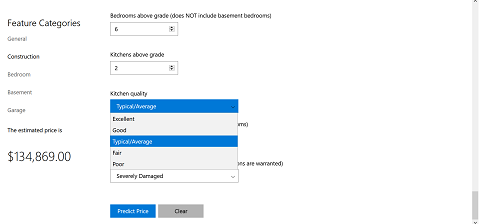
\includegraphics{images/screenshot-04.png}
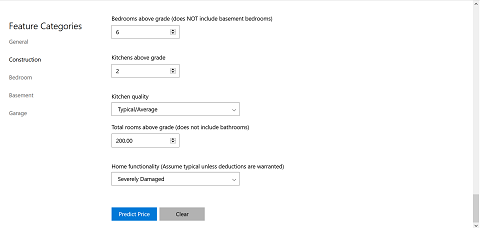
\includegraphics{images/screenshot-03.png}

We were able to build a web application that can predict the price of a
house given certain features. The application runs in the browser and
talks to a flask server that is taking data and passing it to a machine
learning model.

\section{4. Conclusion}\label{conclusion}

There are real world problems that can be solved with machine learning.
Some of these solutions can take real world data and make very accurate
predictions that can be useful to our daily lives. Users can leverage
the power of machine learning without being data scientist when easy to
use applications are built around some of these complicated models.

\section{5. Refrences}\label{refrences}

Pedro Marcelino, \emph{Comprehensive data exploration with Python},
Kaggle, February 2017. Accessed on: April 19, 2021. {[}Online{]}
Available:
\url{https://www.kaggle.com/pmarcelino/comprehensive-data-exploration-with-python}

J. Ade-Ojo, \emph{Predicting House Prices With Machine Learning},
Towards Data Science, Janurary 8, 2021. Accessed on: April 19, 2021.
{[}Online{]} Available:
\url{https://towardsdatascience.com/predicting-house-prices-with-machine-learning-62d5bcd0d68f}

\emph{House Prices - Advanced Regression Techniques}, Kaggle, Accessed
on: April 19, 2021. {[}Online{]} Available:
\url{https://www.kaggle.com/c/house-prices-advanced-regression-techniques}

\emph{House Prices EDA}, Kaggle, Accessed on: April 19, 2021.
{[}Online{]} Available:
\url{https://www.kaggle.com/dgawlik/house-prices-eda}
